%%============
%%  ** Author: Shepherd Qirong
%%  ** Date: 2020-04-23 23:56:59
%%  ** Github: https://github.com/ShepherdQR
%%  ** LastEditors: Shepherd Qirong
%%  ** LastEditTime: 2020-05-25 00:33:35
%%  ** Copyright (c) 2019--20xx Shepherd Qirong. All rights reserved.
%%============

\documentclass[UTF8]{article}
\usepackage{ctex}
\usepackage{multirow,booktabs}
\usepackage{amsmath,amsthm,amsfonts,amssymb,bm,mathrsfs,upgreek } 
\usepackage[paper=a4paper,top=3.5cm,bottom=2.5cm,
left=2.7cm,right=2.7cm,
headheight=1.0cm,footskip=0.7cm]{geometry}
\usepackage{color,graphicx,verbatim}
\RequirePackage{setspace}
\setstretch{1.523}


\usepackage{pgf, tikz}
\usetikzlibrary{arrows, decorations.pathmorphing, backgrounds, positioning, fit, petri, automata}
\definecolor{yellow1}{rgb}{1,0.8,0.2} 





\begin{document}

\section{Introduction}




    Typography,字体设计是矢量的。The Quick Brown Fox Jumps Over The Lazy Dog.

    Rasterization, real time(>=30FPS)
    Curves and curvature
    Ray tracing
    animation simulation
    We learn graphics, not graphics apis.
    需要猜测的是计算机视觉的事情,不是计算机图形学的事情。
    图形学computer graphics 研究model和从model到image。
    计算机视觉computer vision研究image和从image到model。

    "fundamentals of computer graphics" a book.

    integrated development environment
\section{A swift and Brutal introduction to linear algebra}




\begin{figure*}[h]
    \centering
   
    \begin{tikzpicture}[->,>=stealth',shorten >=1pt,auto,node distance=2.8cm, semithick ]
    \tikzstyle{every state}=[shape=rectangle, fill=none, draw=black, text=black]
    \tikzstyle{h1}=[shape=rectangle, fill=none, draw=none, text=black ]
    \tikzstyle{vertex2}=[shape=rectangle, fill=none, draw=none, text=black, text width =2em]
    \tikzstyle{every node}=[font=\small, scale=0.8]

    \node[state]  (s1) at (0,0)    {扫描};
    \node[state]  (s2) at (1.5,0)    {配准};
    \node[state]  (s3) at (3.5,0)    {Octree 更新};
    \node[state]  (s4) at (6,0)    {视点预生成};
    \node[state]  (s5) at (8,0)    {视点评价};
    \node[state]  (s6) at (10,0)    {视点选择};
    \node[state]  (s7) at (12,0)    {路径规划};
    \node[state]  (s8) at (14,0)    {NBV解};

    \path 
    (s1)    edge[->]   node{} (s2)
    (s2)    edge[->]   node{} (s3)      
    (s3)    edge[->]   node{} (s4)
    (s4)    edge[->]   node{} (s5)
    (s5)    edge[->]   node{} (s6)
    (s6)    edge[->]   node{} (s7)
    (s7)    edge[->]   node{} (s8)        
            ;

\end{tikzpicture}

    \caption{zsz}\label{fig:zs}
\end{figure*}













\end{document}













\begin{comment}




\begin{figure*}[h]
    \centering
   
    \begin{tikzpicture}[->,>=stealth',shorten >=1pt,auto,node distance=2.8cm, semithick ]
    \tikzstyle{every state}=[shape=rectangle, fill=none, draw=black, text=black]
    \tikzstyle{h1}=[shape=rectangle, fill=none, draw=none, text=black ]
    \tikzstyle{vertex2}=[shape=rectangle, fill=none, draw=none, text=black, text width =2em]
    \tikzstyle{every node}=[font=\small, scale=0.8]


    \draw (0,0) rectangle (2,2);
    \node[h1]    (s1) at (0, 0)      {视角优化计算};
        \node[vertex2]  (s21) at (2,3){初始帧扫描};
            \node[state]  (s211) at (10,4){初始帧配准};
            \node[state]  (s212) at (10,3){扫描区域与坐标基准选择};
            \node[state]  (s213) at (10,2){点云前处理};






    %\node[vertex]    (s2) at (0, 0)      {基于局部特征的车辆位姿配准};
        \node[state]  (s21) at (5,3){初始帧扫描};
            \node[state]  (s211) at (10,4){初始帧配准};
            \node[state]  (s212) at (10,3){扫描区域与坐标基准选择};
            \node[state]  (s213) at (10,2){点云前处理};


            
        \node[state]  (s22) at (5,0){车辆点云数据库};
            \node[state]  (s221) at (10,1){构建CAD-点云-图案数据库};
            \node[state]  (s222) at (10,0){CAD模型的前处理与点云生成};
            \node[state]  (s223) at (10,-1){点云区域选择与特征计算};

            \node[state]    (s32) at (20, 0)      {基于局部特征的车辆位姿配准};

    \path
    (s22)   edge[bend left=17]  node{} (s221)
            edge[->]   node{} (s222)
            edge[bend right=17]  node{} (s223)
            
            
            ;


\end{tikzpicture}




    \caption{zsz}\label{fig:zs}
\end{figure*}


















\begin{figure*}[h]
    \centering
   
    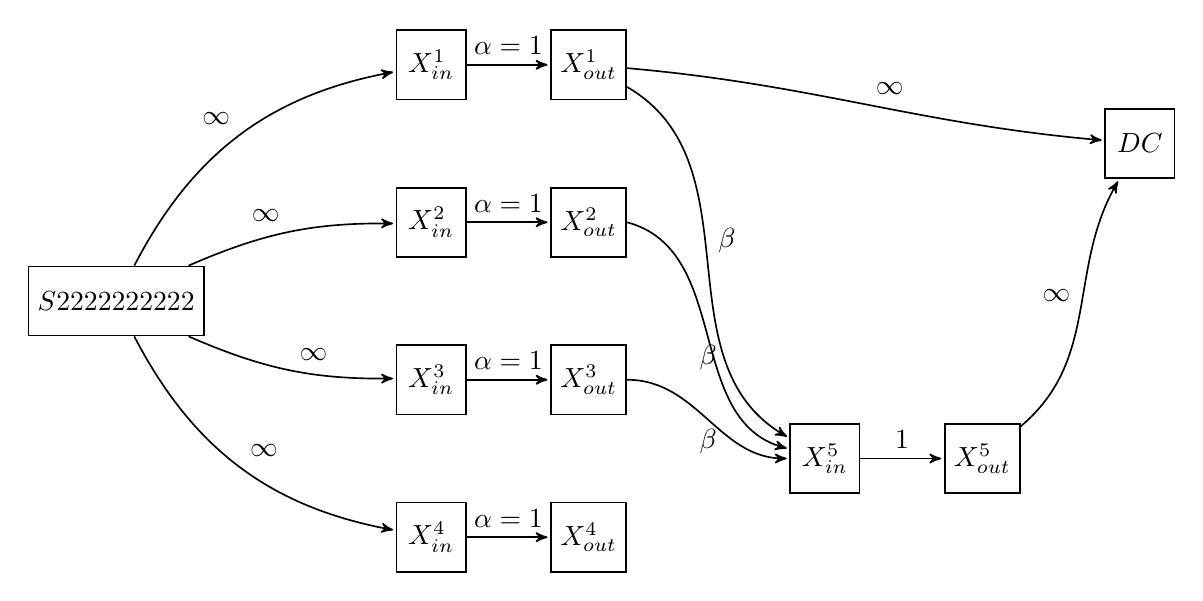
\begin{tikzpicture}[->,>=stealth',shorten >=1pt,auto,node distance=2.8cm, semithick]
    \tikzstyle{every state}=[shape=rectangle, fill=none, draw=black, text=black]

\node[state]         (S) at (-6, 0)              {$S2222222222$};
\node[state]         (xin1) at (-2, 3)           {$X^1_{in}$};
\node[state]         (xin2) at (-2, 1)        {$X^2_{in}$};
\node[state]         (xin3) at (-2, -1)       {$X^3_{in}$};
\node[state]         (xin4) at (-2, -3)           {$X^4_{in}$};
\node[state]         (xout1) at (0, 3)          {$X^1_{out}$};
\node[state]         (xout2) at (0, 1)        {$X^2_{out}$};
\node[state]         (xout3) at (0, -1)   {$X^3_{out}$};
\node[state]         (xout4) at (0, -3)           {$X^4_{out}$};
\node[state]         (xin5)  at (3, -2)   {$X^5_{in}$};
\node[state]         (xout5) at (5, -2)   {$X^5_{out}$};
\node[state]         (DC) at (7, 2)           {$DC$};

\path
(S) edge[bend left=26]  node {$\infty$} (xin1)
    edge[bend left=12]  node {$\infty$} (xin2)
    edge[bend right=12]  node {$\infty$} (xin3)
    edge[bend right=26]  node {$\infty$} (xin4)
(xin1) edge  node {$\alpha=1$} (xout1)
(xin2) edge  node {$\alpha=1$} (xout2)
(xin3) edge  node {$\alpha=1$} (xout3)
(xin4) edge  node {$\alpha=1$} (xout4)
(xin5) edge  node {$1$} (xout5);

\draw[->] (xout1) to[out=-30,in=150] node {$\beta$} (xin5);
\draw[->] (xout2.east) to[out=-15,in=165] node [below] {$\beta$} (xin5);
\draw[->] (xout3.east) to[out=0,in=180] node [below] {$\beta$} (xin5.west);
\draw[->] (xout1) to[out=-5,in=175] node {$\infty$} (DC);
\draw[->] (xout5) to[out=40, in=-120] node {$\infty$} (DC);
\end{tikzpicture}




    \caption{zz}\label{fig:z}
\end{figure*}




\end{comment}